\chapter{User's Manual} \label{sec:manual}

This manual will describe the impedance spectrometer in detail and give step by step instructions for using it.


\section{Overview}

An overview of the device connections can be seen in Figure \ref{fig:device_connections}. Connector footprints for
unimplemented features are not labeled, the push buttons on the board are the same as those on the
STM32F4 Discovery board.

\begin{figure}[htb]
  \centering
    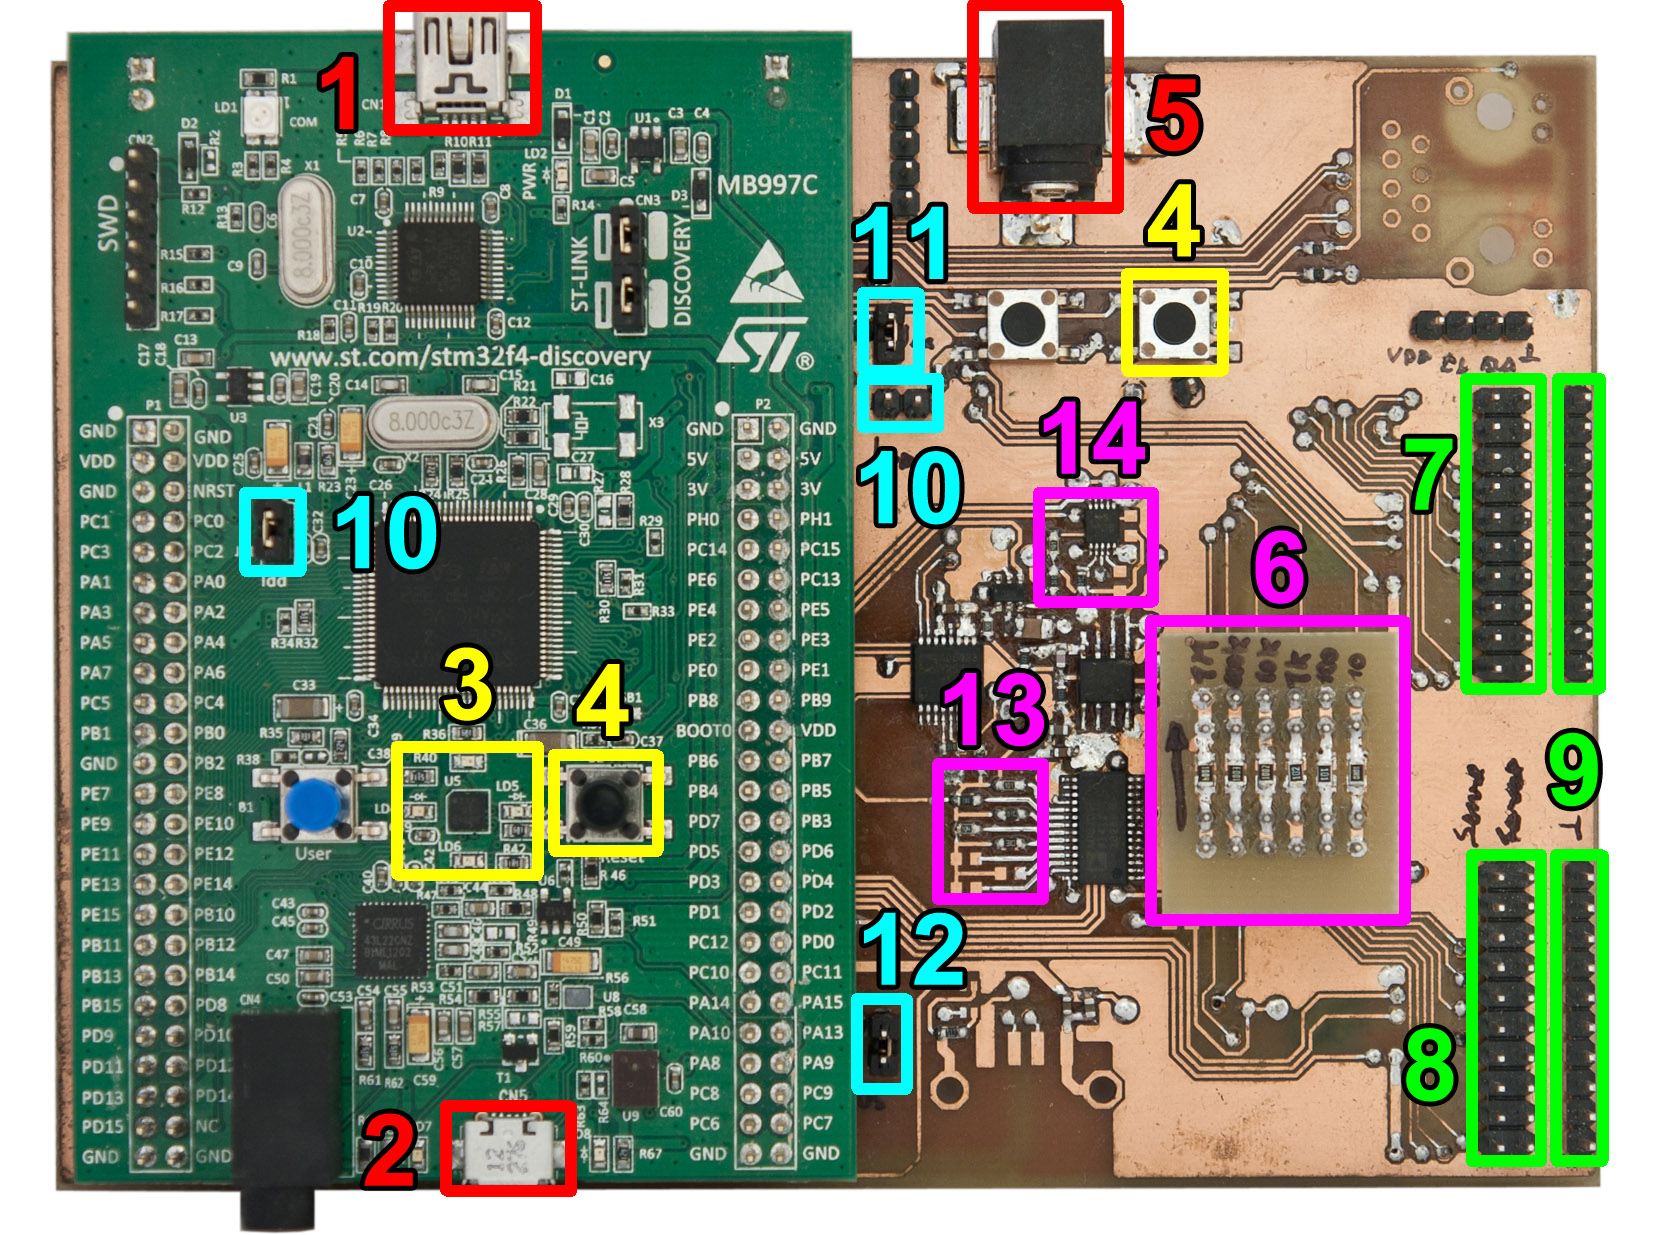
\includegraphics[width=\textwidth]{bilder/device_connections.jpg}
  \caption[Interface on the assembled impedance spectrometer]{
    Interface on the assembled impedance spectrometer:
    \begin{enumerate*}[label=\textbf{\arabic*}, itemjoin={{ -- }}]
      \item \label{itm:usb_prog}  USB programming and power connector
      \item \label{itm:usb_dev}   device USB connector
      \item \label{itm:leds}      status LEDs
      \item \label{itm:btn_rst}   reset button
      \item \label{itm:dc_jack}   DC power jack
      \item \label{itm:r_cal}     board with calibration resistors
      \item \label{itm:meas_out}  measurement output connections, sense (left) and force (right)
      \item \label{itm:meas_in}   measurement input connections (same as output)
      \item \label{itm:meas_gnd}  ground connections
      \item \label{itm:jump_idd}  $ I_\text{DD} $ measurement jumper
      \item \label{itm:jump_icc}  $ I_\text{CC} $ measurement jumper
      \item \label{itm:jump_vbus} $ V_\text{BUS} $ jumper
      \item \label{itm:r_fb}      feedback resistors
      \item \label{itm:r_att}     attenuation resistors
    \end{enumerate*} }
  \label{fig:device_connections}
\end{figure}

The USB programming connector \ref{itm:usb_prog} is used to program and debug the device, it can also be used to power
the device from a standard phone charger or similar supply with a Mini-B USB plug.
The device USB connector \ref{itm:usb_dev} is used to connect the device to a PC and control it.
The DC jack \ref{itm:dc_jack} is a standard \unit{2.5}{\milli\meter} jack (center positive) and can be used to
power the device with a \unit{5}{\volt} DC supply.

When using the device with an external power supply, or powered from the programming connector \ref{itm:usb_prog},
the $ V_\text{BUS} $ jumper \ref{itm:jump_vbus} may be disconnected to prevent the board from drawing power from the
device connector \ref{itm:usb_dev}.

The jumpers \ref{itm:jump_idd} and \ref{itm:jump_icc} can be used to measure the current consumption of the
microcontroller and all the other parts, respectively (note that there are two jumpers for $ I_\text{DD} $,
one on the STM32F4 Discovery board and one on the board, and care should be taken to use only one).

There are four status LEDs \ref{itm:leds}, three of which are used at this time:
\begin{itemize}
	\item \textbf{\color{blue} blue} will blink when the device is powered on, indicating that the firmware
    hasn't locked up,
  \item \textbf{\color{OliveGreen} green} will light up while a measurement is in progress, allowing the user
    to see when it has finished,
  \item \textbf{\color{red} red} will be turned on in case of an error in the firmware, this means the device
    should be reset using the reset button \ref{itm:btn_rst} and the steps leading up to the error should be
    documented, allowing the programmer to fix it.
\end{itemize}

\subsection{First Steps}

Before powering up the device for the first time, the following things should be checked:
\begin{itemize}
	\item the STM32F4 discovery board is properly connected,
  \item a board with calibration resistors is connected to the calibration pins \ref{itm:r_cal},
  \item the necessary feedback and attenuation resistors \ref{itm:r_fb} and \ref{itm:r_att} are soldered on,
  \item the current measurement jumpers \ref{itm:jump_idd} and \ref{itm:jump_icc} are connected
    (or a current meter of course),
  \item the $ V_\text{BUS} $ jumper \ref{itm:jump_vbus} is connected when no external power supply is used.
\end{itemize}

After connecting the device to a PC, any application that can access a serial port can be used to communicate with it.
Settings such as baud rate or parity don't matter.
When not using the MATLAB functions (see \autoref{sec:matlab}), the device is configured via a simple virtual console
interface using human readable commands. By typing \command{help}, a list of possible commands and their
explanations can be displayed.

The following steps assume the device is fitted with an EEPROM for configuration storage.
The first thing to do after assembling the device is to configure the fitted calibration and feedback resistors, as well
as possible attenuations and the coupling capacitor time constant using the \command{setup} command:
\begin{itemize}
	\item enter possible output voltage attenuations in the order they are selected with the attenuation multiplexer:
    \command{setup attenuation <values>...}
  \item enter feedback resistor values in the order they are connected to the feedback multiplexer in ohms:
    \command{setup feedback <values>...}
  \item enter calibration resistor values in the order they are soldered on the little resistor board (right to left):
    \command{setup calibration <values>...}
  \item enter the coupling capacitor time constant in ms (calculated by $ C_\text{coupl} \cdot \unit{1.1}{\kilo\ohm} $):
    \command{setup coupl <milliseconds>}
\end{itemize}
Typing \command{help setup} shows other options for the \command{setup} command, however none of them are currently
used since the respective peripherals are not yet implemented.

By typing \command{board info}, general information for the whole board is displayed, which includes the configured
resistors and attenuation values.


\section{Making Measurements}

After the first steps have been completed, measurements can be performed.

First, the unknown impedance(s) need to be connected to the output and input connectors \ref{itm:meas_out} and
\ref{itm:meas_in}. When a four-wire connection is not used, the two output and input pins, respectively, need to be
connected nonetheless for proper operation.

\subsection{Sweep Configuration}

Then, the sweep parameters need to be configured. This is done using the \command{board set} command with the following
parameters (only those that should be changed need to be sent):
\begin{itemize}
	\item \command{--start=FREQ} and \command{--stop=FREQ} set the start and stop frequency of the sweep in \hertz.
    Note that when setting start and stop frequency in a single command, an error can occur when the new start
    frequency is equal to or higher than the previous stop frequency. In this case you need to change the order in
    which start and stop options appear on the command line.
  \item \command{--steps=NUM} sets the number of frequency steps in a sweep, that is the number of times the frequency
    is incremented.
  \item \command{--settl=NUM} sets the number of settling cycles (see \autoref{sec:ad5933_proc}). The valid range is
    0--511 and can be extended 2 or 4 times by specifying a multiplier like \command{x2}. For example, valid values
    would be \command{20} or \command{40x2}, but not \command{512} (use \command{256x2} instead).
  \item \command{--voltage=RANGE} sets the output voltage range in \milli\volt. The possible ranges are determined by
    the configured attenuation values, they are one of the AD5933 output voltages (\unit{200}{\milli\volt},
    \unit{400}{\milli\volt}, \unit{1}{\volt} or \unit{2}{\volt}) divided by one of the attenuation values. For example,
    if attenuation values of 1 and 100 were configured, the possible voltage ranges would be 2000, 1000, 400, 200, 20,
    10, 4 and 2.
  \item \command{--gain=(on|off)} sets whether the input gain stage (PGA) is enabled. When enabled, the input signal is
    amplified by a factor of 5 prior to sampling.
  \item \command{--feedback=OHMS} sets the used feedback resistor, this needs to be one of the configured values.
\end{itemize}
The current value for any parameter can be displayed with the \command{board get} command, which accepts one of the
parameters and displays its value (for example \command{board get start} would display the start frequency in \hertz).
A quick overview of the current values can be displayed by typing \command{board get all}, which displays all sweep
parameters in a format suitable for parsing by PC software.

When selecting range settings, the following procedure should be used:
\begin{itemize}
	\item Set the output voltage low enough so the output current does not exceed \unit{10}{\milli\ampere} with the
    lowest impedance expected.
  \item Set the current feedback resistor to a value low enough so the input voltage stays below 3V for the highest
    output current expected.
  \item If necessary, the PGA can be enabled to further amplify the input voltage when high impedances are to be
    measured. For accurate results, the input signal should be close to 3V for the lowest impedance expected.
\end{itemize}

\subsection{Calibration}

Before measurements can be made the system has to be calibrated with a known impedance (see \autoref{sec:ad5933_proc}
on why this is necessary). After the range settings (start and stop frequency, output voltage, feedback resistor or
PGA gain) are changed, the \command{board calibrate} command is used to do that. The calibration impedance, specified
as the only parameter to the command, should be in the same range as the impedance to be measured for accurate results.

A recalibration is also necessary when the ambient temperature changes significantly.

Normally, calibration resistors are connected to the device with the small PCB \ref{itm:r_cal} mounted on the
calibration connectors. However, these connectors are just measurement connectors like \ref{itm:meas_out} and
\ref{itm:meas_in}, so calibration resistors can also be connected without a dedicated calibration resistor board.
\emph{Note that resistors should always be used for calibration, because the calibration impedance must not introduce
  a phase shift of its own.}

\subsection{Starting a Sweep}

Once the sweep parameters are set and a calibration has been performed, a sweep can be started.
Typing \command{board start} with the desired port number as the only parameter will initiate a sweep, indicated by
the green LED \ref{itm:leds} lighting up. The port number determines which pair of pins will be used, with the topmost
pins having the number 0 and the bottom pins the number 9. The valid range can also be displayed with the
\command{board info} command.

While a sweep is running, the status can be displayed by typing \command{board status}. This will print whether or not
the sweep is still running and the number of points measured.

A running measurement can be stopped by typing \command{board stop}, which also resets the AD5933 and disconnects the
output and input pins. To disconnect the outputs when no measurement is running \command{board standby} can be used.

\subsection{Reading Results}

After a sweep is finished, the measurement results can be read with the \command{board read} command.
The format in which measurement data is transferred can either be set permanently with the
\command{board set --format=FMT} command, or specified to the \command{board read} command for a single transfer.

The format specification is a set of flags, represented by uppercase letters. There are two modes for data transfer,
ASCII and binary. All possible flags can be found in \autoref{tab:format_flags}.

When using binary format, at least one of the \texttt{P} and \texttt{C} flags has to be specified. The \texttt{H} flag
causes the number of bytes to follow to be transferred at the start of the transmission as an unsigned \unit{32}{bit}
integer. The frequency is also transferred as an unsigned \unit{32}{bit} integer, the impedance values (magnitude and
angle, or real and imaginary parts) as single precision \unit{32}{bit} floating point values.

When using ASCII format, at least one of the \texttt{P} and \texttt{C} flags, one of the \texttt{F} and \texttt{X}
flags, as well as one of three separator flags have to be specified. The data is transferred in human readable form,
one line per record, with values separated by the specified separator character. After the last record, two line breaks
are sent to signal the end of the transmission. The \texttt{H} flag causes a header line to be transferred before the
first record.

\begin{table}[htpb]
  \caption{Possible format flags for transferring measurement data.}
  \centering
  \begin{tabular}{>{\ttfamily\bgroup}l<{\egroup}|p{10cm}}
    Flag  & Function \\ \hline
    A     & Selects ASCII transfer format \\
    B     & Selects binary transfer format \\ \hline
    P     & Selects polar number format (magnitude in ohms and angle in radians) \\
    C     & Selects Cartesian number format (real and imaginary parts in ohms) \\ \hline
    H     & When present, a header is printed for ASCII format, or the byte count is transferred for binary format \\ \hline
    F     & ASCII only: impedance values are printed as formatted floating point values, the frequency as an unsigned integer \\
    X     & ASCII only: frequency and impedance values are printed as hexadecimal values \\ \hline
    S     & ASCII only: Selects a space character as the separator \\
    T     & ASCII only: Selects a tab character as the separator \\
    D     & ASCII only: Selects a comma character as the separator
  \end{tabular}
  \label{tab:format_flags}
\end{table}
